\documentclass[10pt,twocolumn]{article}

% use the oxycomps style file
\usepackage{oxycomps}

% read references.bib for the bibtex data
\bibliography{references}

% include metadata in the generated pdf file
\pdfinfo{
    /Title (Comps Project Ethical Considerations)
    /Author (Roberto Villegas Jr.)
}

% set the title and author information
\title{Comps Project Ethical Considerations}
\author{Roberto Villegas Jr.}
\affiliation{Occidental College}
\email{rvillegas@oxy.edu}

\begin{document}

\maketitle

\section{Context}

The project that these ethical considerations are about is a web application that aims to centralize information about League of Legends (LoL for short) Esports in one place.
This web app will use the APIs of different LoL websites around the web and store this data in a constantly-updated database.
This project's front end will make a call to the database, which the database sends the appropriate information to the front end.

Some of the information this web app will handle is pro player information (bio, current/former teams, achievements, etc.), pro team information (current roster, previous/current matches, coaching staff, etc.), league information (teams, standings, schedule, etc.), and a spectator link for those that want to watch pro players while they are playing on the LoL public servers.
The spectator will work by using LoL's built-in spectator mode; the web app will only provide the link required for this to work.
This project also plans on including a notification system for users to stay up-to-date with their favorite players and teams (more on this later).

To get an idea of what this project would look like, you can look at pretty much any fan-made wiki sites.
This project certainly will have an original layout and navigation system, but the general idea of having a website display information in an easy-to-read format will remain the same or close to the same.

\section{Accessibility}

The largest and most important ethical concern about the project is its accessibility.
Since the purpose of the project is to display information to users, the project's priority must be to consider how different people digest information.
This has less to do with a user's preferences and more to do with a user's ability to digest information.
For example, a user with "perfect" vision can easily read a web page with information while a blind user won't know anything about the web page unless it includes and incorporates audio features.
Even a user's access to technology must be considered, requiring the project to be accessible to multiples devices instead of only one.
The three different areas of accessibility the project must pay attention to are visually impaired user, users with physical disabilities, and device limitations.

\subsection{Visually Impaired Users}

It is obvious how a visually impaired user will have trouble using web app like this one, especially if there were no features to enable their accessibility.
It is important to note that there are more than just blindness; colorblindness, partial blindness, and much more are things that need to be considered in order to make the web app truly accessible for anyone with a visual impairment.

The American Foundation for the Blind's (AFB for short) website lists plenty of tips to help web developers make their websites more accessible for those with visual impairments \cite{AFBAccessibilityResources}.
First, making a website keyboard accessible will make it plenty easier for these users to navigate through the website \footnote{\url{https://www.afb.org/consulting/afb-accessibility-resources/keyboard-accessibility}}.
Keyboard navigation is the "traditional" approach to website for visually impaired users, so designing the website with keyboard tools in mind is important.
For example, one should be mindful about the design of the Document Object Model for the website, since screen readers will rely on this to read the website contents in the order that they appear in the DOM.
Failure to properly order its contents can make information on the website confusing for the user.
Additionally, the AFB suggests to use native HTML controls in order since these are an "established standard". Attempting to use different controls might make it more difficult to differentiate parts of the website and overcomplicate website navigation.

The AFB also outlines how effective image and video descriptions can be in a website.
Since a user's tools won't be able to "read" an image or video, additional text is required for the reader to figure out what is being shown.
For images, this is done in the form of alternative (alt for short) text \footnote{\url{https://www.afb.org/consulting/afb-accessibility-resources/improving-your-web-site}}.
These texts are brief and highlight important information about what the image is showing.
Putting essential information and context into an alt text makes the difference between a good and bad alt text.
For example, an alt text that says "business man in a suit" does not have the same effect as "Bill Gates, co-founder of Microsoft".
For videos, the inclusion of "audio description" fulfills the same purpose \footnote{\url{https://www.afb.org/consulting/afb-accessibility-resources/video-description}}.

Lastly, the colors used by the website matters to those with impairments affected by color (such as those with colorblindness).
Using colors without much contrast can make it hard to make out what a website is saying, or figure out where different buttons or other tools are.
Color choice is important when making a website, and can open the website up to more people who want to use it.

\subsection{Users with Physical Disabilities}

The project should also consider users that may physically struggle to navigate it.
Alternative devices designed for the physically disabled already exist, such as things like modified keyboard (fewer keys, larger keys, etc.) and Lomak keyboards (light-activated device mounted on a user's head, see Figure \ref{fig:LomakKeyboard}).
Still, a responsible and ethical programmer will make sure to still include web app features to ensure that everyone has equal access and use to the project.

\begin{figure}[ht!]
    \centering
    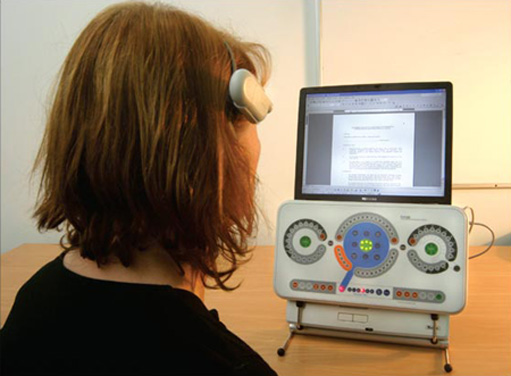
\includegraphics[width=.95\linewidth]{LomakKeyboard.jpg}
    \caption{
        Lomak Keyboard in use.
    }
    \label{fig:LomakKeyboard}
\end{figure}

% Links unable to be added due to error
The Web Content Accessibility Guidelines (WCAG for short) outlines how developers can make their web product more accommodating for those with disabilities, including physical disabilities \cite{WCAG2point1}.
For example, there is a guideline that explains how pointer cancellation should work with a single-pointer operation of a web app. % Link 1: https://www.w3.org/TR/WCAG21/#pointer-cancellation
This is specifically to help those that might input something they don't intend on inputting, and allowing them to continue viewing whatever page they're on instead of changing pages and struggling to get back to where they were.
There is also a guideline that sets a minimum "target size" for page elements so that things are not too small and impossible to click on. % Link 2: https://www.w3.org/TR/WCAG21/#target-size

Additional adjustments can be done by creating a separate layout aimed at helping users with physical disabilities. The main action of this feature would be to create bigger buttons and use the previously mentioned guidelines so that users will be able to click on buttons and navigate through the page without much struggle. 

\section{Privacy}

These days, one of the biggest concerns for users is their privacy.
Any and all data collected and stored by any software must be held ethically and with the express consent of the user.
The current plans of this project include an "account" system that allows users to create an account with their favorite preferences such as favorite teams, players, leagues, etc.
It will also have the capability of sending notifications to the user either through email or (possibly) text, which is where the focus for privacy comes in.

To give users control of their private information, an email or phone number will not be required when making an account.
The notification feature will be entirely optional, and any user that only wants to access the information in the web app from time to time will be able to do so privately.
Additionally, a user can use this web app without making an account, essentially allowing anonymous users.

\section{Security}

Although there is not a significant amount of sensitive information that must be protected in this project, a good security system is still required so that a user's information does not get use improperly or maliciously.
Handling a user's information with care is a responsibility of a developer, and this project is no exception.

Firstly, usernames and passwords must be stored and transported securely.
This means making sure this information is encrypted from the user's end as well as in the database.
A simple hash function somewhere in between the front end and the back end should be able to provide some security for this.
This will also help with email addresses and phone numbers.

\section{Closing}

Based on these considerations, it is possible for this project to be entirely done ethically.
As long as the proper adjustments are made for accessibility, anyone will be able to use this website and learn from the information it displays.
As the project moves along, there will certainly be more features that can be included to make it even easier for people to use.
For now, these issues are sufficiently taken care of and the project may continue its development confidently.

\printbibliography

\end{document}
